\chapter{fractions.h Documentation}
\ifsingle
\maketitle
\fi
\chaptermeta[draft][2025-09-10]
\section{Introduction}\label{sec:intro}
\texttt{fractions.h} provides a toolbox for reconstructing interfaces from the
volume fraction field. Its two main purposes are:

\begin{enumerate}
  \item \textbf{Initialization} --- assigning volume fraction values from a given
  level-set field. This step is used to define the initial condition in VOF
  methods. In addition, it can generate face fraction values to ensure a closed
  interface, which is specifically required by embedded boundary methods.
  \item \textbf{Reconstruction} --- rebuilding the interface from the volume
  fraction field for use in VOF advection. Unlike initialization, this
  reconstruction does not require the interface to be closed.
\end{enumerate}

In addition, the header includes auxiliary functions to support coarsening and refinement of volume fractions across grid levels, visualization of the interface, and computation of the total interface area.

\subsection{Assigning Volume Fractions from Level-Set Fields}\label{sec:fractions-init}  

Level-set function $\Phi$ represents the distance to the interface and are stored discretely at vertices of the gird. Take $\Phi$ as input the function \func{fractions} computes the volume fraction field and face fraction (if required). Space where $\Phi>0$ is deemed as inside the interface, the volume fraction is set to $1.0$ and vice versa.

In header file \texttt{geometry.h} a group of tools have been constructed to obtain volume fractions of single cell given the interface normal $\mathbf{n}$ and the intersection $\alpha$ both in 2D and 3D cases. The overall process to compute volume fraction is therefore twofolds: 1)to obtain $(\mathbf{n}, \alpha)$ 2)pass the parameter to corresponding tools provided by \texttt{geometry.h}. The underlying theory shall be briefly introduced in the following.

\begin{figure}[H]
  \centering
  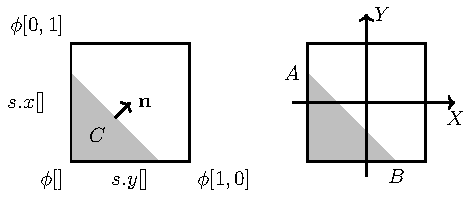
\includegraphics[height=5cm]{./image/fractions-h/normal.pdf}
  \caption{A sketch for level-set based volume fraction initialization. The left panel shows the normal vector $\mathbf{n}$, face fraction $s$ and the vertex level-set value. The right panel illustrates the coordinate system, two intersection point is marked as $A,B$.}
  \label{fig:fractions-normal}
\end{figure}

Figure \ref{fig:fractions-normal} illustrates the geometry of a single cell in 2D. In the left panel the level-set values at the four vertices are denoted as $\phi[]$, $\phi[1,0]$, $\phi[0,1]$ and $\phi[1,1]$. The nonzero face fractions (edge fraction for 3D cases) are $s.x[]$ and $s.y[]$ which can be obtained directly from the level-set values as $s.x[] = \frac{\phi[]}{\phi[]-\phi[1,0]}$ and $s.y[] = \frac{\phi[]}{\phi[]-\phi[0,1]}$. 

Consider that $\oint_{\partial \Omega}\mathbf{n}dl = 0$ which equals to
\begin{equation}
  \mathbf{n} + (s.x[1]-s.x[])\mathbf{e_x} + (s.y[1]-s.y[])\mathbf{e_y} = 0
\end{equation}
Hence the interfacial normal is $\mathbf{n} = (s.x[]-s.x[1],s.y[]-s.y[1])$, the interfacial normal can be computed following same formula with $s$ representing the face fraction on six cell-faces. 

As for $\alpha$, it can be derived from the intersection points $A$ and $B$ in the right panel of figure \ref{fig:fractions-normal}. Consider the origin locates at cell center and the length of the cell as $1$, coordinates of $A$ and $B$ are $(-0.5,s.y[]-0.5),(s.x[]-0.5,-0.5)$ respectively. The line equation of the interface is $n_x X + n_y Y = \alpha$ where $\mathbf{n} = (n_x,n_y)$, substituting the coordinates of $A$ or $B$ into the equation yields (A as an example)
\begin{equation}  
  \alpha = -0.5n_x + n_y (s.y[]-0.5)
\end{equation}
The final $\alpha$ is determined by averaging the results from $A$ and $B$. For 3D cases, the procedure to compute $\alpha$ is the same but with more complicity, since one plane can cut through a cube with minimum three intersection points and maximum six intersection points.

To summarize, the algorithm to compute volume fractions from level-set fields is as follows:
\begin{enumerate}
  \item Compute face (edge) fractions from level-set values at vertices.
  \item Compute interfacial normal $\mathbf{n}$ from face (edge) fractions.
  \item Compute intersection $\alpha$ from $\mathbf{n}$ and face (edge) fractions.
  \item Compute volume (face) fraction from $\mathbf{n}$ and $\alpha$ using tools provided by \texttt{geometry.h} (2D cases ends here).
  \item For 3D cases, compute interfacial normal using face fractions in all three directions, then compute $\alpha$ from $\mathbf{n}$ and edge fractions, finally compute volume fraction using tools provided by \texttt{geometry.h}.
\end{enumerate}

\section{Functions}

\subsection{Refinement Functions}

Functions \func{fraction\_refine} and \func{alpha\_refine} are used to refine the volume fraction field and the intersection field $\alpha$, respectively, when tree grids are employed and a cell is subdivided.

Starting from the parent interfacial cell, the volume fraction $c$, the interface normal $\mathbf{n}$, and the intersection value $\alpha$ are computed sequentially using tools provided in \texttt{myc.h} and \texttt{geometry.h}. The volume fractions of the child cells are then obtained using the function \func{rectangle\_fraction} (see the \texttt{geometry.h} documentation for details). For instance, when provided with the sub-rectangle $(0,0,0)$--$(0.5,0.5,0.5)$, the function returns the volume fraction contained within this region. By specifying the indices of child cells (e.g., $child.i = \pm 1$), the function iterates through all sub-cells by rotating the interfacial normal, i.e. by multiplying $\mathbf{n}$ with the child indices.

The refinement of $\alpha$ for child cells can be understood as a coordinate transformation. Specifically, the origin is shifted to the center of the child cell and the unit length is scaled by a factor of $1/2$. Starting from the parent cell representation
\begin{equation}
  n_x X + n_y Y + n_z Z = \alpha,
\end{equation}
the transformed equation for the child cell, using the coordinate transformation
$X' = 2\bigl(X - \tfrac{1}{2} child.x\bigr)$, becomes
\begin{equation}
  n_x X' + n_y Y' + n_z Z' =
  2\alpha - \tfrac{n_x child.x}{2} - \tfrac{n_y child.y}{2}
        - \tfrac{n_z child.z}{2} = \alpha'
\end{equation}
